% Investment memo. Numbers come from generated/metrics.tex and generated/tables/*.tex.
\documentclass[11pt,a4paper]{article}
\usepackage[top=21mm,bottom=21mm,left=25mm,right=25mm,footskip=9mm]{geometry}
\usepackage{style/quantedge}
\usepackage{natbib}
\usepackage{placeins}
\urlstyle{same}
\setcitestyle{authoryear,round,aysep={},yysep={,}}
\setlength{\bibsep}{2.5pt plus 0.5pt}
\renewcommand{\bibfont}{\small}
% Generated by scripts/generate_report_data.py from the verified reference. Do not edit.

\newcommand{\qeBundle}{1c7bd6007fe22b014b25}
\newcommand{\qeDataset}{qe1\_20050101\_20261030\_r3\_6c4633a7ba}
\newcommand{\qeConfigHash}{587ddbe363589fb6956c23c5fe8b2b544bac81d9224a0b4bb59f60f5fbc0a017}
\newcommand{\qeProtocolCommit}{782ec20}
\newcommand{\qeHurdle}{6.75\%}
\newcommand{\qeSpending}{4.00\%}
\newcommand{\qeInflation}{2.50\%}
\newcommand{\qeFee}{0.25\%}
\newcommand{\qeRealGrowth}{0.00\%}
\newcommand{\qeHorizon}{10}
\newcommand{\qeBudgetVarNinetyFive}{1.00\%}
\newcommand{\qeBudgetVar}{1.50\%}
\newcommand{\qeBudgetEs}{2.00\%}
\newcommand{\qeBudgetVol}{10.00\%}
\newcommand{\qeBudgetDrawdown}{20.00\%}
\newcommand{\qeBudgetScenario}{20.00\%}
\newcommand{\qeBudgetVarUsd}{\$150,000}
\newcommand{\qeBudgetEsUsd}{\$200,000}
\newcommand{\qeBudgetDrawdownUsd}{\$2,000,000}
\newcommand{\qeDevCagr}{6.65\%}
\newcommand{\qeDevVol}{8.77\%}
\newcommand{\qeDevDrawdown}{−22.18\%}
\newcommand{\qeDevSharpe}{0.70}
\newcommand{\qeSelCagr}{10.38\%}
\newcommand{\qeSelVol}{7.74\%}
\newcommand{\qeSelDrawdown}{−14.47\%}
\newcommand{\qeSelSharpe}{1.14}
\newcommand{\qeEvalCagr}{7.63\%}
\newcommand{\qeEvalVol}{8.80\%}
\newcommand{\qeEvalDrawdown}{−16.78\%}
\newcommand{\qeEvalSharpe}{0.51}
\newcommand{\qeFullCagr}{7.68\%}
\newcommand{\qeFullVol}{8.58\%}
\newcommand{\qeFullDrawdown}{−22.18\%}
\newcommand{\qeFullSharpe}{0.72}
\newcommand{\qeEvalCagrSixty}{8.41\%}
\newcommand{\qeEvalVolSixty}{10.66\%}
\newcommand{\qeEvalDrawdownSixty}{−20.77\%}
\newcommand{\qeEvalSharpeSixty}{0.50}
\newcommand{\qeEvalCagrEqual}{13.69\%}
\newcommand{\qeFullBeta}{0.29}
\newcommand{\qeFullAlpha}{3.13\%}
\newcommand{\qeEvalAlpha}{0.77\%}
\newcommand{\qeHurdleGapDev}{−0.10\%}
\newcommand{\qeIncomeYield}{2.19\%}
\newcommand{\qeIncomeMean}{1.80\%}
\newcommand{\qeRealReturn}{4.88\%}
\newcommand{\qeCpiInflation}{2.59\%}
\newcommand{\qeSharpeAccrual}{0.719}
\newcommand{\qeSharpePrimary}{0.723}
\newcommand{\qeVar}{1.54\%}
\newcommand{\qeEs}{2.03\%}
\newcommand{\qeVarUsd}{\$153,950}
\newcommand{\qeEsUsd}{\$203,169}
\newcommand{\qeVarExcess}{\$3,950}
\newcommand{\qeEsExcess}{\$3,169}
\newcommand{\qeVarNinetyFive}{0.87\%}
\newcommand{\qeNormalVarNinetyFive}{0.90\%}
\newcommand{\qeFullVar}{1.63\%}
\newcommand{\qeFullEs}{2.50\%}
\newcommand{\qeFullEsUsd}{\$250,185}
\newcommand{\qeNormalVar}{1.29\%}
\newcommand{\qeNormalEs}{1.49\%}
\newcommand{\qeMcVar}{1.28\%}
\newcommand{\qePotEs}{2.03\%}
\newcommand{\qePotVar}{1.56\%}
\newcommand{\qeFullPotEs}{2.50\%}
\newcommand{\qeMcDraws}{25,000}
\newcommand{\qeHsFullExceptions}{65}
\newcommand{\qeFullSessions}{4,987}
\newcommand{\qeHsFullUc}{0.040}
\newcommand{\qeHsFullInd}{$1.7\times10^{-5}$}
\newcommand{\qeHsEvalUc}{0.394}
\newcommand{\qeHsEvalInd}{0.216}
\newcommand{\qeHsEvalExceptions}{18}
\newcommand{\qeNormalEvalExceptions}{27}
\newcommand{\qeNormalEvalUc}{0.004}
\newcommand{\qeEvalSessions}{1,464}
\newcommand{\qeBaselHs}{4}
\newcommand{\qeBaselNormal}{9}
\newcommand{\qeBaselHsZone}{green}
\newcommand{\qeBaselNormalZone}{yellow}
\newcommand{\qeBaselStart}{3 Nov 2025}
\newcommand{\qeBaselEnd}{30 Oct 2026}
\newcommand{\qeBaselExpected}{2.5}
\newcommand{\qeWeightSpy}{20.4\%}
\newcommand{\qeShareSpy}{29.6\%}
\newcommand{\qeWeightAgg}{40.0\%}
\newcommand{\qeShareAgg}{7.0\%}
\newcommand{\qeWeightGld}{25.0\%}
\newcommand{\qeShareGld}{31.6\%}
\newcommand{\qeWeightXle}{14.6\%}
\newcommand{\qeShareXle}{31.8\%}
\newcommand{\qeDivWeighted}{3.30\%}
\newcommand{\qeDivWeightedUsd}{\$329,643}
\newcommand{\qeDivBenefit}{38\%}
\newcommand{\qeCorrSpyAgg}{0.00}
\newcommand{\qeCorrSpyGld}{0.07}
\newcommand{\qeCorrSpyXle}{0.70}
\newcommand{\qeDriftSessions}{2,771}
\newcommand{\qeActiveSessions}{4,987}
\newcommand{\qeDriftMax}{45.14\%}
\newcommand{\qeDriftTicker}{AGG}
\newcommand{\qeDriftDate}{23 Oct 2008}
\newcommand{\qeDriftEquity}{37.30\%}
\newcommand{\qeGfcReturn}{−8.93\%}
\newcommand{\qeGfcDrawdown}{−23.87\%}
\newcommand{\qeGfcUsd}{\$892,991}
\newcommand{\qeGfcReturnSixty}{−29.99\%}
\newcommand{\qeGfcDrawdownSixty}{−30.33\%}
\newcommand{\qeCovidReturn}{−16.23\%}
\newcommand{\qeCovidDrawdown}{−18.84\%}
\newcommand{\qeCovidUsd}{\$1,622,750}
\newcommand{\qeCovidReturnSixty}{−20.59\%}
\newcommand{\qeCovidDrawdownSixty}{−20.81\%}
\newcommand{\qeRatesReturn}{−6.57\%}
\newcommand{\qeRatesDrawdown}{−13.36\%}
\newcommand{\qeRatesUsd}{\$656,660}
\newcommand{\qeRatesReturnSixty}{−20.58\%}
\newcommand{\qeRatesDrawdownSixty}{−20.63\%}
\newcommand{\qeHypoReturn}{−4.48\%}
\newcommand{\qeHypoDrawdown}{−4.48\%}
\newcommand{\qeHypoUsd}{\$447,652}
\newcommand{\qeHypoReturnSixty}{−19.80\%}
\newcommand{\qeHypoDrawdownSixty}{−19.80\%}
\newcommand{\qeFlags}{307}
\newcommand{\qeFlagNegative}{188}
\newcommand{\qeFlagJump}{101}
\newcommand{\qeFlagBreak}{18}
\newcommand{\qePriceSessions}{5,492}
\newcommand{\qeReturnSessions}{5,491}
\newcommand{\qeMissingCells}{0}
\newcommand{\qeVintages}{5,142}
\newcommand{\qeRfObservations}{5,493}
\newcommand{\qeRfSupported}{3,617}
\newcommand{\qeRfInferred}{1,537}
\newcommand{\qeRfFallback}{314}
\newcommand{\qeRfDocumented}{23}
\newcommand{\qeRfUnresolved}{2}
\newcommand{\qeHurdleGapDevAbs}{0.10}
\newcommand{\qeIncomeGapUsd}{\$180,617}
\newcommand{\qeEvtRecentXi}{0.054}
\newcommand{\qeEvtFullXi}{0.254}
\newcommand{\qeEvtRecentN}{63}
\newcommand{\qeEvtFullN}{274}
\newcommand{\qeEvtSparseN}{31}
\newcommand{\qeDevBootVarLow}{1.31\%}
\newcommand{\qeDevBootVarHigh}{1.75\%}
\newcommand{\qeDevBootEsLow}{1.75\%}
\newcommand{\qeDevBootEsHigh}{2.70\%}
\newcommand{\qeDevBootFinite}{62}
\newcommand{\qeBaselSelHs}{10}
\newcommand{\qeBaselSelNormal}{14}
\newcommand{\qeHsSelInd}{$8.4\times10^{-4}$}
\newcommand{\qeHsFullExpected}{49.9}
\newcommand{\qeHsEvalExpected}{14.6}
\newcommand{\qeAllocEqualEs}{2.99\%}
\newcommand{\qeAllocSixtyEs}{2.50\%}

\hypersetup{pdftitle={Quant Edge: Investment Committee Memo},pdfauthor={Quant Edge research team}}
\qefooter{Quant Edge 1.0 \textbar\ Investment committee memo \textbar\ Evidence to 30 Oct 2026}
\newcommand{\qetable}[3]{%
  \begin{table}[#1]\centering\caption{#2}\small #3\end{table}}
\newcommand{\qefigure}[4][\linewidth]{%
  \begin{figure}[#2]\centering\includegraphics[width=#1]{generated/figures/#3.pdf}\caption{#4}\label{fig:#3}\end{figure}}
\setcounter{topnumber}{2}
\setcounter{totalnumber}{3}
\renewcommand{\topfraction}{0.9}
\renewcommand{\textfraction}{0.08}
\renewcommand{\floatpagefraction}{0.8}

\begin{document}
\thispagestyle{fancy}
\qekicker{Serendib University Endowment \textperiodcentered{} USD 10 million \textperiodcentered{} Investment committee memo}\par\vspace{2pt}
{\sffamily\bfseries\huge\color{qeink} Keep the rule, change the terms\par}\vspace{3pt}
{\sffamily\small\color{qemuted} Quant Edge research team. Evidence frozen at 30 October 2026. Bundle \qeBundle. Independent human validation is pending.\par}
\qedecision{Proposed decision: conditional ADJUST}{Retain the seven-fund universe and the registered constrained minimum-variance rule as a candidate, but do not commit capital. The committee should first settle the spending plan, the loss budgets and the holdings-drift policy. This is a team proposal under a competition brief. No university committee has reviewed it.}

The endowment wants to preserve capital, generate income and grow in real terms, and the committee believes that ``avoiding large losses is more important than maximizing gains'' \citep{quantedge2026}. We therefore test one registered rule against an explicit funding hurdle and explicit loss budgets, and report where it falls short.

\begin{table}[h]\centering\caption{The decision in five pieces of evidence}\label{tab:evidence}\small
\begin{tabular}{@{}p{0.235\textwidth}p{0.325\textwidth}p{0.385\textwidth}@{}}
\toprule
Question & Evidence & Reading \\
\midrule
Does it fund the mission? & CAGR \qeDevCagr{} / \qeSelCagr{} / \qeEvalCagr{} in development, selection and evaluation, against a \qeHurdle{} hurdle & Cleared in two of three periods, and missed by \qeHurdleGapDevAbs{} points in development. \\
Does income cover spending? & Ending path yield \qeIncomeYield{} against \qeSpending{} spending & No. Spending also needs planned sales. \\
How bad is a bad day? & VaR \qeVarUsd{} and ES \qeEsUsd{} at 99\%, against \qeBudgetVarUsd{} and \qeBudgetEsUsd{} & Above budget by \qeVarExcess{} and \qeEsExcess{}. Full-history ES is \qeFullEsUsd{}. \\
How bad is a crisis? & GFC replay endpoint \qeGfcReturn{}, drawdown \qeGfcDrawdown{} & Endpoint is within the \qeBudgetScenario{} scenario budget; the drawdown is not. \\
Can we trust the model? & Latest 250 sessions: \qeBaselHs{} exceptions, \qeBaselHsZone{}. Full history: \qeHsFullExceptions{} against \qeHsFullExpected{} expected & Recent results are acceptable; the full-history model rejects on frequency and independence. \\
\bottomrule
\end{tabular}
\end{table}

No allocation we tested meets every proposed limit. The candidate is the only one inside the target caps, and it sits marginally above its tail budgets. Those excesses are small and estimated with error, so they do not justify rejecting the rule. They do justify refusing to call the mandate acceptable as proposed, because funding, tail risk and governance remain open together.

\section{Mandate, return hurdle and risk budget}
The brief fixes the client, the USD 10 million scale and the seven eligible funds. It leaves the horizon, return objective and risk constraints to each team. Everything in \cref{tab:mandate} is therefore our proposal, recorded before post-2016 strategy results were inspected. None of it is a client or organiser requirement.

\begin{table}[htb]\centering\caption{Proposed mandate assumptions and daily loss budgets}\label{tab:mandate}\small
\begin{tabular}{@{}ll@{\hspace{2.2em}}lrr@{}}
\toprule
Assumption & Proposal & Budget & Share of NAV & USD \\
\midrule
Horizon & \qeHorizon{} years & Historical VaR 95\%, 1 day & \qeBudgetVarNinetyFive & \$100,000 \\
Spending & \qeSpending{} of opening NAV & Historical VaR 99\%, 1 day & \qeBudgetVar & \qeBudgetVarUsd \\
Inflation & \qeInflation{} a year & Historical ES 99\%, 1 day & \qeBudgetEs & \qeBudgetEsUsd \\
Extra mandate fee & \qeFee{} a year & Annual volatility & \qeBudgetVol & --- \\
Real growth & \qeRealGrowth & Drawdown, scenario loss & \qeBudgetDrawdown & \qeBudgetDrawdownUsd \\
\bottomrule
\end{tabular}
\end{table}

With spending and the fee deducted against opening NAV, the hurdle $R$ satisfies
\begin{equation}
1 + R - s - f = (1 + \pi)(1 + g).
\end{equation}
At zero real growth this gives $R = s + f + \pi =$ \qeHurdle{}. It is a planning sum, not a return forecast, and we attach no probability to it. ETF expenses are already inside adjusted returns, so the \qeFee{} is a separate proposed mandate cost rather than a second fund expense. The return paths below deduct trading costs but not spending or this fee.

A review budget is a line that triggers a committee discussion. It is not a guarantee that losses stop there.

\section{Data quality and its limits}
Prices are dividend- and split-adjusted closes for all seven ETFs from Yahoo Finance, on the expected NYSE session grid: \qePriceSessions{} prices and \qeReturnSessions{} one-session returns from 4 January 2005, with \qeMissingCells{} missing price cells. Missing sessions would invalidate both adjacent returns rather than be filled. The audit retained all \qeFlags{} quality flags (\qeFlagNegative{} large negatives, \qeFlagJump{} robust jumps and \qeFlagBreak{} candidate breaks). Flags are prompts for review, and none was deleted. Log returns support statistical diagnostics, and simple returns are used for portfolio arithmetic, dollar losses and tail models because weighted log returns do not aggregate exactly. Augmented Dickey-Fuller tests reject a unit root in strategy returns, which supports stationarity of the level but says nothing about independence or constant volatility.

The risk-free proxy is the DTB3 discount quote \citep{fredDtb3}, versioned across all \qeVintages{} published ALFRED vintages. Of \qeRfObservations{} observations, \qeRfSupported{} have availability supported by a vintage, \qeRfDocumented{} rest on Federal Reserve notices, \qeRfInferred{} are inferred from later vintages and may be over-delayed, \qeRfFallback{} use a labelled sparse-era calendar fallback, and \qeRfUnresolved{} remain unresolved. Exact historical release hours are unverified, so this is day-level evidence and not exact point-in-time data. Dividing the quote by 252 is a proxy for a bill return, and a 91-day accrual sensitivity moves the full-period Sharpe ratio only from \qeSharpePrimary{} to \qeSharpeAccrual{}. CPI \citep{fredCpi} is revised, is used only as ex-post context, and lacks October 2025 and October 2026 values. ETF prices come from one provider and were not independently verified across the whole history.

\section{Portfolio construction}
Markowitz's framework \citep{markowitz1952} underlies the rule, but expected returns are the least reliable input and optimisation gains can be lost to estimation error \citep{demiguel2009}. We therefore use the minimum-variance portfolio, which needs no return forecast. Each month the rule uses the prior 504 sessions and a sample covariance to set a long-only, fully invested target, with each ETF at most 40\% and equities at most 35\%. Those caps imply that AGG and GLD each sit between 25\% and 40\% at target, and equities between 20\% and 35\%, so a more defensive portfolio is unreachable. Those bounds follow from our caps and are not a view on gold.

\qefigure[0.74\linewidth]{htb}{target_path}{Monthly targets, 2007--2026. Target weights only: holdings drift between rebalances. Candidate rule, estimated on the prior 504 sessions.}

Weights for session $t$ are fixed before its return, holdings then drift, and trades cost 5~bp per unit of traded weight. Commit \texttt{\qeProtocolCommit} recorded the rule and proposed mandate before post-2016 strategy results were viewed. Development ends in 2016, selection covers 2017--2020 and evaluation starts in 2021. No selection-period winner was chosen and nothing was retuned afterwards. Whole-history asset analysis and fixed-exposure stress work had already been seen, so this is a registered-rule evaluation and not a blinded experiment.

The caps bind on monthly targets, not on daily holdings. Holdings passed at least one target cap on \qeDriftSessions{} of \qeActiveSessions{} sessions, reaching \qeDriftMax{} in \qeDriftTicker{} on \qeDriftDate{} and \qeDriftEquity{} in equities. Continuous compliance is not claimed. Concentration also runs deeper than weights show: SPY already contains energy and technology, and the \qeWeightXle{} XLE position is an optimiser outcome, not a macro view.

\section{Performance, income and funding}
\qefigure{htb}{wealth_drawdown}{Net wealth and drawdown of the historical strategy paths, 5 January 2007 to 30 October 2026, after a 504-session warm-up. Investable-rule paths with drifting holdings, net of trading costs, before spending and the extra fee. Drawdown includes starting wealth.}

\Cref{tab:periods} keeps all three frozen samples together. Showing evaluation alone would flatter the rule: its \qeEvalCagr{} clears the hurdle, but development's \qeDevCagr{} does not. Against 60/40 the rule gave up return in evaluation (\qeEvalCagr{} against \qeEvalCagrSixty{}) for lower volatility and a shallower drawdown, leaving Sharpe ratios almost equal at \qeEvalSharpe{} and \qeEvalSharpeSixty{}. Equal weight earned \qeEvalCagrEqual{} in that period, far more than the candidate, while breaching our caps. We report that and do not switch to it, because choosing the realised winner would defeat the protocol.

\begin{table}[htb]\centering\caption{Frozen samples, net of trading costs. References need not meet the candidate's caps.}\label{tab:periods}\small\begin{tabular}{@{}llS[table-format=2.2]S[table-format=2.2]S[table-format=-2.2]S[table-format=1.2]r@{}}
\toprule
Period & Portfolio & {CAGR (\%)} & {Vol.\ (\%)} & {Max DD (\%)} & {Sharpe} & Sessions \\
\midrule
Development & Candidate rule & 6.65 & 8.77 & -22.18 & 0.70 & 2,516 \\
 & Equal weight & 5.45 & 17.71 & -43.26 & 0.35 &  \\
 & 60/40 & 6.07 & 12.19 & -35.78 & 0.49 &  \\
\midrule
Selection & Candidate rule & 10.38 & 7.74 & -14.47 & 1.14 & 1,007 \\
 & Equal weight & 10.90 & 15.50 & -27.94 & 0.66 &  \\
 & 60/40 & 11.73 & 12.07 & -21.63 & 0.87 &  \\
\midrule
Evaluation & Candidate rule & 7.63 & 8.80 & -16.78 & 0.51 & 1,464 \\
 & Equal weight & 13.69 & 12.89 & -17.49 & 0.80 &  \\
 & 60/40 & 8.41 & 10.66 & -20.77 & 0.50 &  \\
\bottomrule
\end{tabular}
\end{table}

Over the full active history (\cref{tab:kpis}) the candidate has a CAPM beta of \qeFullBeta{} to SPY \citep{sharpe1964}. Its Jensen alpha of \qeFullAlpha{} is an in-sample regression statistic, and it falls to \qeEvalAlpha{} in evaluation, so it is not evidence of persistent skill. The information ratio is negative because the rule deliberately holds less equity than 60/40. A defensive mandate should expect that.

\begin{table}[htb]\centering\caption{Full active history, 5 January 2007 to 30 October 2026. CAPM uses SPY; ratios use the versioned risk-free proxy. Information ratio is unavailable for 60/40 against itself.}\label{tab:kpis}\small\begin{tabular}{@{}lS[table-format=-2.2]S[table-format=-2.2]S[table-format=-2.2]@{}}
\toprule
Full active history & {Candidate rule} & {Equal weight} & {60/40} \\
\midrule
Net CAGR (\%) & 7.68 & 8.91 & 7.88 \\
Annual volatility (\%) & 8.58 & 15.98 & 11.73 \\
Downside deviation (\%) & 6.07 & 11.37 & 8.33 \\
Maximum drawdown (\%) & -22.18 & -43.26 & -35.78 \\
Sharpe ratio & 0.72 & 0.52 & 0.57 \\
Sortino ratio & 1.02 & 0.73 & 0.81 \\
Calmar ratio & 0.35 & 0.21 & 0.22 \\
CAPM beta to SPY & 0.29 & 0.76 & 0.59 \\
Jensen alpha, annual (\%) & 3.13 & 0.19 & 0.43 \\
Treynor ratio & 0.21 & 0.11 & 0.11 \\
Tracking error to 60/40 (\%) & 8.16 & 6.85 & 0.00 \\
Information ratio to 60/40 & -0.06 & 0.22 & {\textit{n/a}} \\
\bottomrule
\end{tabular}
\end{table}

\begin{minipage}[t]{0.56\textwidth}\vspace{0pt}
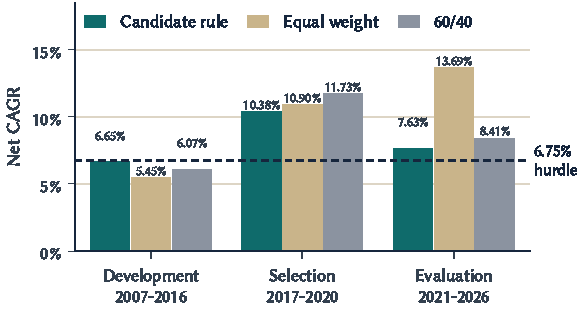
\includegraphics[width=\linewidth]{generated/figures/funding.pdf}
\captionof{figure}{Net CAGR against the proposed hurdle, on frozen samples.}\label{fig:funding}
\end{minipage}\hfill
\begin{minipage}[t]{0.40\textwidth}\vspace{0pt}
\subsection{Return is not spendable income}
The path's ending cash yield is \qeIncomeYield{} (mean \qeIncomeMean{}), below \qeSpending{} spending. On USD 10 million that gap is about \qeIncomeGapUsd{} a year, illustratively.
\end{minipage}

\vspace{4pt}
That yield describes the historical path and is not an exact yield on today's target. Distributions are already inside adjusted returns and are never added twice. Total-return spending is workable, but it means selling assets, possibly in a drawdown, so it needs an approved liquidity plan. In real terms the path grew \qeRealReturn{} a year before spending over common complete months against \qeCpiInflation{} CPI inflation. That interval differs from the frozen samples, and it is not a forecast.

\section{Tail risk: how bad, and how sure}
All estimates in \cref{tab:risk} share one exposure (the prospective target at the final close), one horizon (one day, before costs) and matched samples. Losses are positive fractions of NAV. We report ES as well as VaR because VaR is silent about losses beyond its quantile and is not subadditive in general, while ES averages the tail and is coherent \citep{artzner1999,acerbi2002}. For a loss budget that matters: ES is the number that asks how bad the bad days are.

\begin{table}[htb]\centering\caption{One-day loss estimates at the prospective target. \textit{n/a}: pure POT is unavailable below its empirical tail boundary.}\label{tab:risk}\footnotesize\setlength{\tabcolsep}{3.4pt}\begin{tabular}{@{}lS[table-format=1.2]S[table-format=1.2]S[table-format=1.2]S[table-format=1.2]S[table-format=1.2]S[table-format=1.2]S[table-format=1.2]S[table-format=1.2]@{}}
\toprule
 & \multicolumn{4}{c}{Recent 1,260 sessions} & \multicolumn{4}{c@{}}{Full 5,491 sessions} \\ \cmidrule(lr){2-5}\cmidrule(l){6-9} & \multicolumn{2}{c}{95\%} & \multicolumn{2}{c}{99\%} & \multicolumn{2}{c}{95\%} & \multicolumn{2}{c@{}}{99\%} \\
\% of NAV & {VaR} & {ES} & {VaR} & {ES} & {VaR} & {ES} & {VaR} & {ES} \\
\midrule
Historical & 0.87 & 1.30 & 1.54 & 2.03 & 0.88 & 1.42 & 1.63 & 2.50 \\
Normal & 0.90 & 1.14 & 1.29 & 1.49 & 0.97 & 1.22 & 1.38 & 1.59 \\
Normal Monte Carlo & 0.90 & 1.14 & 1.28 & 1.49 & 0.97 & 1.23 & 1.38 & 1.59 \\
Pure POT-GPD & 0.87 & 1.30 & 1.56 & 2.03 & {\textit{n/a}} & {\textit{n/a}} & 1.68 & 2.50 \\
Body/tail hybrid & 0.87 & 1.30 & 1.56 & 2.03 & 0.88 & 1.42 & 1.68 & 2.50 \\
\bottomrule
\end{tabular}
\end{table}

\qefigure{htb}{tail_models}{VaR and ES at 99\% on matched samples and the same target weights, with the proposed budgets. Normal Monte Carlo samples the same Normal model.}

\subsection{Why the models disagree}
At 99\% on the recent sample, Historical VaR is \qeVar{} and Normal VaR is \qeNormalVar{}. The gap is about the shape of the tail: the Normal curve is fitted to all days, and it understates the worst ones. Normal ES of \qeNormalEs{} lies well below Historical ES of \qeEs{}. Normal Monte Carlo (\qeMcDraws{} draws) gives \qeMcVar{}: it agrees with Normal up to sampling error because it samples the same distribution, so it is a check and not a fat-tail model. At 95\%, by contrast, Normal VaR of \qeNormalVarNinetyFive{} is above Historical at \qeVarNinetyFive{}. The Normal model is not uniformly optimistic, only wrong about shape.

The sample matters as much as the model. The recent window starts in October 2021 and omits the GFC and COVID-19, and full-history ES of \qeFullEs{} is much higher than the recent \qeEs{}. Neither is the true number. The recent window reflects current conditions but has not seen a major liquidity crisis, while the full window contains crises but mixes regimes and applies today's weights to a past that held different ones. The committee should read them as a range.

\subsection{Extreme value theory: where extrapolation starts}
The Pickands--Balkema--de Haan result motivates fitting a Generalised Pareto Distribution to losses above a high threshold $u$ \citep{balkema1974,pickands1975,davison1990}. For $N_u$ excesses in $n$ observations, with $\hat p_u = N_u/n$ and confidence $c$ in the fitted tail,
\begin{equation}
\mathrm{VaR}_c = u + \frac{\beta}{\xi}\left[\left(\frac{1-c}{\hat p_u}\right)^{-\xi} - 1\right], \qquad
\mathrm{ES}_c = \frac{\mathrm{VaR}_c + \beta - \xi u}{1 - \xi} \quad (\xi < 1).
\end{equation}

Threshold choice trades bias against variance \citep{scarrott2012}: a lower threshold keeps more data but reaches into the body of the distribution. The inherited policy fixed the 95\% quantile before fitting, required at least 50 strict excesses and never lowered the threshold to rescue a fit. That gives \qeEvtRecentN{} excesses with $\xi$ of \qeEvtRecentXi{} on the recent sample and \qeEvtFullN{} with $\xi$ of \qeEvtFullXi{} on the full history (\cref{tab:evt}). The recent 97.5\% candidate has only \qeEvtSparseN{} excesses, so its fit is unavailable. Shape estimates rise with the threshold in the full sample (\cref{fig:evt_stability}), so they are not clearly stable, and we do not claim the threshold is uniquely right.

\begin{table}[htb]\centering\caption{Threshold diagnostics at the prospective target. Modified scale is $\beta-\xi u$.}\label{tab:evt}\footnotesize\begin{tabular}{@{}lrrrrrl@{}}
\toprule
Sample & Quantile (\%) & Excesses & Shape $\xi$ & Scale $\beta$ (\%) & Modified scale (\%) & Status \\
\midrule
Recent & 90.0 & 126 & 0.113 & 0.339 & 0.266 & Fitted \\
Recent & 92.5 & 94 & 0.093 & 0.364 & 0.295 & Fitted \\
Recent & 95.0 & 63 & 0.054 & 0.407 & 0.360 & Fitted \\
Recent & 97.5 & 31 & \textit{n/a} & \textit{n/a} & \textit{n/a} & Below 50 excesses \\
\midrule
Full history & 90.0 & 549 & 0.193 & 0.384 & 0.269 & Fitted \\
Full history & 92.5 & 411 & 0.247 & 0.370 & 0.192 & Fitted \\
Full history & 95.0 & 274 & 0.254 & 0.405 & 0.181 & Fitted \\
Full history & 97.5 & 137 & 0.389 & 0.394 & −0.075 & Fitted \\
\bottomrule
\end{tabular}
\end{table}

\qefigure{htb}{evt_stability}{Threshold stability at the prospective target. Intervals are iid asymptotic, ignore dependence and threshold choice, and are shown for orientation only.}

Pure POT VaR at 99\% is \qePotVar{}, with ES \qePotEs{} recent and \qeFullPotEs{} full history, close to Historical in both. So EVT here confirms the empirical tail and does not add a far worse estimate. A positive fitted shape is consistent with heavy tails under this model, but on its own it is not a formal rejection of the Gaussian. EVT also assumes stable, roughly independent excesses, which clustered markets violate; conditional approaches exist \citep{mcneil2000} and are not used here. Pure POT is unavailable below its tail boundary, including 95\% on the full history, where ties put the boundary just above 95\%. The hybrid uses the empirical body there and is labelled separately. It is not EVT extrapolation.

\begin{minipage}[t]{0.40\textwidth}\vspace{0pt}
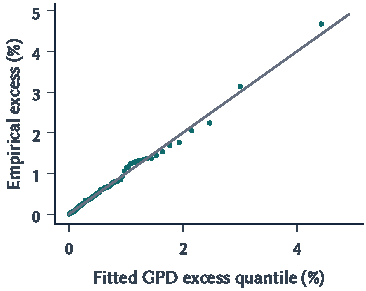
\includegraphics[width=\linewidth]{generated/figures/development_qq.pdf}
\captionof{figure}{Development-only QQ plot, different exposure from \cref{tab:evt}.}\label{fig:qq}
\end{minipage}\hfill
\begin{minipage}[t]{0.56\textwidth}\vspace{0pt}
\subsection{Earlier development-only evidence}
Step 7 studied a different exposure (SPY 33.93\%, AGG 40.00\%, GLD 26.07\%) on data through 2016 only. Its moving-block bootstrap (block 10, 100 replications) gave pure-POT 99\% intervals of \qeDevBootVarLow{} to \qeDevBootVarHigh{} for VaR and \qeDevBootEsLow{} to \qeDevBootEsHigh{} for ES. At 95\% only \qeDevBootFinite{} of 100 replicates were usable, so that interval stays unavailable.
\end{minipage}

\vspace{4pt}
Those intervals show how wide tail uncertainty can be, but they are not confidence bands for today's target, and the QQ plot is descriptive rather than a proof of fit. They suggest, without establishing it for this exposure, that an ES excess of \qeEsExcess{} is small relative to plausible estimation error. We treat it as a reason for review, not a precisely measured breach.

\section{Model validation: forecast first, then observe}
Each day's VaR uses only the prior 500 sessions and the holdings known before that day, and it is compared with that day's gross loss, for \qeFullSessions{} sessions. Kupiec's test asks whether exceptions occur at the right rate \citep{kupiec1995}. Christoffersen's asks whether they cluster \citep{christoffersen1998}. Historical simulation is the primary model and Normal is a fixed comparison. Rolling Monte Carlo and EVT results are not claimed.

\qefigure{htb}{exceptions}{Historical VaR 99\% against realised gross loss, using actual pre-return holdings (top). Rolling count of exceptions in 250 sessions, with expected 2.5 and Basel-style yellow and red bands (bottom).}

\begin{table}[htb]\centering\caption{99\% coverage tests. Non-rejection is not proof of safety; sparse samples have low power.}\label{tab:backtest}\footnotesize\begin{tabular}{@{}llrrrrrr@{}}
\toprule
99\% VaR & Model & Sessions & Exceptions & Expected & Kupiec $p$ & Indep.\ $p$ & Cond.\ $p$ \\
\midrule
Full active & Historical & 4,987 & 65 & 49.9 & 0.040 & $1.7\times10^{-5}$ & $1.2\times10^{-5}$ \\
 & Normal & 4,987 & 105 & 49.9 & $8.2\times10^{-12}$ & $2.2\times10^{-7}$ & $1.0\times10^{-16}$ \\
\midrule
Development & Historical & 2,516 & 32 & 25.2 & 0.188 & 0.007 & 0.011 \\
 & Normal & 2,516 & 53 & 25.2 & $1.2\times10^{-6}$ & $9.0\times10^{-5}$ & $3.5\times10^{-9}$ \\
\midrule
Selection & Historical & 1,007 & 15 & 10.1 & 0.145 & $8.4\times10^{-4}$ & 0.001 \\
 & Normal & 1,007 & 25 & 10.1 & $6.9\times10^{-5}$ & 0.023 & $2.7\times10^{-5}$ \\
\midrule
Evaluation & Historical & 1,464 & 18 & 14.6 & 0.394 & 0.216 & 0.323 \\
 & Normal & 1,464 & 27 & 14.6 & 0.004 & 0.012 & $6.4\times10^{-4}$ \\
\bottomrule
\end{tabular}
\end{table}

The evidence in \cref{tab:backtest} is mixed, and we do not resolve it in the rule's favour. In evaluation, Historical 99\% does not reject at 5\% (Kupiec $p$ of \qeHsEvalUc{}, independence $p$ of \qeHsEvalInd{}), with \qeHsEvalExceptions{} exceptions against \qeHsEvalExpected{} expected. Over the full history it rejects on both frequency ($p$ of \qeHsFullUc{}) and independence ($p$ of \qeHsFullInd{}), with \qeHsFullExceptions{} exceptions against \qeHsFullExpected{} expected. Failures arrive together, as expected from a slowly updating 500-day window when volatility jumps (\cref{fig:exceptions}). Normal is worse at 99\%: \qeNormalEvalExceptions{} evaluation exceptions and a Kupiec $p$ of \qeNormalEvalUc{}.

\begin{table}[htb]\centering\caption{Educational Basel-style 99\% results for the final 250 sessions of each frozen sample.}\label{tab:basel}\small\begin{tabular}{@{}lllrl@{}}
\toprule
Period & Model & Final 250-session block & Exceptions & Zone \\
\midrule
Development & Historical & 6 Jan 2016 -- 30 Dec 2016 & 2 & \qezone{green} \\
 & Normal & 6 Jan 2016 -- 30 Dec 2016 & 3 & \qezone{green} \\
\midrule
Selection & Historical & 7 Jan 2020 -- 31 Dec 2020 & 10 & \qezone{red} \\
 & Normal & 7 Jan 2020 -- 31 Dec 2020 & 14 & \qezone{red} \\
\midrule
Evaluation & Historical & 3 Nov 2025 -- 30 Oct 2026 & 4 & \qezone{green} \\
 & Normal & 3 Nov 2025 -- 30 Oct 2026 & 9 & \qezone{yellow} \\
\bottomrule
\end{tabular}
\end{table}

The latest Basel-style block, \qeBaselStart{} to \qeBaselEnd{}, shows \qeBaselHs{} Historical exceptions (\qeBaselHsZone{}) and \qeBaselNormal{} Normal exceptions (\qeBaselNormalZone{}) against \qeBaselExpected{} expected \citep{bcbs1996}. That green light is real but narrow. The final block of the selection sample, which includes COVID-19, was red for both models (\qeBaselSelHs{} and \qeBaselSelNormal{} exceptions), as \cref{tab:basel} shows. These zones are a teaching diagnostic, not regulatory approval, and a calm year says little about the next crisis.

\section{Risk budget, allocation and stress}
ES and VaR are homogeneous, so Euler allocation splits total risk into position contributions that sum exactly to the total \citep{tasche2008}. \Cref{tab:contributions} shows the current target on the recent sample. AGG is \qeWeightAgg{} of capital but \qeShareAgg{} of Historical ES, while XLE is \qeWeightXle{} of capital and \qeShareXle{} of ES. GLD contributes \qeShareGld{}, so its defensive label does not make it a tail hedge in this sample. Shares are local to one sample, and a small share is not guaranteed protection.

\begin{table}[htb]\centering\caption{Euler contributions at 99\%, recent 1,260 sessions. Zero-weight ETFs omitted. Components sum to total Historical ES.}\label{tab:contributions}\small\begin{tabular}{@{}lS[table-format=3.1]S[table-format=1.2]S[table-format=1.2]S[table-format=3.1]S[table-format=3.1]@{}}
\toprule
ETF & {Weight (\%)} & {Marginal (\%)} & {Component (\%)} & {Hist.\ share (\%)} & {Normal share (\%)} \\
\midrule
SPY & 20.4 & 2.95 & 0.60 & 29.6 & 26.2 \\
AGG & 40.0 & 0.36 & 0.14 & 7.0 & 13.3 \\
GLD & 25.0 & 2.57 & 0.64 & 31.6 & 36.7 \\
XLE & 14.6 & 4.42 & 0.65 & 31.8 & 23.7 \\
\midrule
\textit{Total} & 100.0 &  & 2.03 & 100.0 & 100.0 \\
\bottomrule
\end{tabular}
\end{table}

\qefigure[0.62\linewidth]{!ht}{weights_risk}{Capital against tail risk: weight is not risk. Prospective target, recent Historical ES at 99\%.}

\begin{table}[htb]\centering\caption{Allocation evidence: Historical simulation, recent 1,260 sessions, proposed tail budgets.}\label{tab:allocations}\small\begin{tabular}{@{}lS[table-format=1.2]S[table-format=1.2]ll@{}}
\toprule
Allocation & {VaR 99 (\%)} & {ES 99 (\%)} & Target caps & Tail budgets \\
\midrule
Candidate rule & 1.54 & 2.03 & \qewithin & \qeabove \\
Equal weight & 2.21 & 2.99 & \qeabove & \qeabove \\
60/40 & 1.89 & 2.50 & \qeabove & \qeabove \\
\bottomrule
\end{tabular}
\end{table}

\Cref{tab:allocations} is why the decision is ADJUST. Equal weight (ES \qeAllocEqualEs{}) and 60/40 (ES \qeAllocSixtyEs{}) both breach the target caps and sit further above the tail budgets. The candidate alone meets the caps and comes closest, but it does not pass. We have not searched for a modified rule that passes: any such rule needs its own registered test, and evaluation data cannot select it. The natural next test is a small, pre-specified trim of the XLE and GLD risk share, with the return it gives up reported.

\qefigure[0.93\linewidth]{!ht}{stress}{Prospective target weights bought and held through actual return paths, and a one-step hypothetical shock. Ex-post exposure replays, not the strategy's historical record. Dashed line: proposed 20\% review level.}

\begin{table}[!ht]\centering\caption{Crisis replay and hypothetical shock on USD 10 million, at prospective target weights.}\label{tab:stress}\small\begin{tabular}{@{}lS[table-format=-2.2]S[table-format=-2.2]rS[table-format=-2.2]S[table-format=-2.2]@{}}
\toprule
 & \multicolumn{3}{c}{Candidate target} & \multicolumn{2}{c@{}}{60/40} \\ \cmidrule(lr){2-4}\cmidrule(l){5-6}
Scenario & {Endpoint (\%)} & {Drawdown (\%)} & Endpoint loss & {Endpoint (\%)} & {Drawdown (\%)} \\
\midrule
Global Financial Crisis & -8.93 & -23.87 & \$892,991 & -29.99 & -30.33 \\
COVID-19 shock & -16.23 & -18.84 & \$1,622,750 & -20.59 & -20.81 \\
2022 rate shock & -6.57 & -13.36 & \$656,660 & -20.58 & -20.63 \\
Hypothetical stagflation & -4.48 & -4.48 & \$447,652 & -19.80 & -19.80 \\
\bottomrule
\end{tabular}
\end{table}

\Cref{tab:stress} separates endpoints from troughs because they answer different questions. In the GFC the target ends at \qeGfcReturn{} after a deepest drawdown of \qeGfcDrawdown{}, which breaches the proposed \qeBudgetDrawdown{} drawdown budget. A liquidity plan must survive the trough, not the endpoint. The target lost less than 60/40 in all three historical crises. The hypothetical stagflation shock (SPY, EFA and EEM $-$25\%, AGG $-$12\%, GLD $+$10\%, XLE $+$20\%, XLK $-$30\%) is our construction, with no assigned duration or probability. Its gold and energy gains are assumptions, not hedges to rely on, and it cannot be compared with one-day ES.

\FloatBarrier
\section{Decision, conditions and monitoring}
Our proposal is conditional ADJUST. We would not accept the mandate as proposed, because tail budgets, income and drift are unresolved. We would not reject it either, because the rule is feasible, its excesses are small, and it lost less than 60/40 in these crises. Three conditions should be met before capital is committed:

\begin{enumerate}
\item \textbf{Funding.} Approve a total-return spending and liquidity plan, or lower spending, given the income gap and a hurdle missed in one of three samples.
\item \textbf{Loss budgets.} Confirm budgets as committee decisions, then test a pre-specified feasible reallocation. Limits must not be raised merely so that the portfolio passes.
\item \textbf{Drift.} Decide whether monthly target control is acceptable, or validate a tighter policy separately.
\end{enumerate}

\begin{table}[htb]\centering\caption{Proposed monitoring triggers. Thresholds are team proposals for committee approval.}\label{tab:monitoring}\small\begin{tabular}{@{}p{0.27\textwidth}rp{0.56\textwidth}@{}}
\toprule
Metric & Threshold & Proposed response \\
\midrule
Historical ES 99\%, one day & 2.00\% & Escalate to committee and assess feasible redistribution; no automatic cap relaxation. \\
Drawdown from peak & 20.00\% & Escalate spending/liquidity and allocation review. \\
Total equity weight & 35.00\% & Flag drift; review at scheduled monthly rebalance, no unapproved daily clipping. \\
Quarterly independence test & $p<0.05$ & Statistical p-value below 0.05 triggers model/dependence review, not proof of future loss. \\
\bottomrule
\end{tabular}
\end{table}

\subsection{What this analysis does not capture}
Past results are not forecasts, and neither capital protection nor sustainable spending is guaranteed. Liabilities and cash-flow timing are not modelled, and off-universe hedges and cash reserves are excluded. Bonds can lose value when rates rise, and gold pays no contractual income. Costs are a flat rate at closing prices, with no market impact, intraday slippage or tax. Foreign-market ETFs close with US trading, so daily correlations reflect non-synchronous underlying markets. Tail estimates assume the past is informative about the future tail, and small differences around a budget are not statistically sharp.

\section{Reproducibility, sources and review status}
The repository holds the frozen data, pinned Python 3.11 dependencies, tests, the verified result bundle \qeBundle{} and the Streamlit app, which runs offline with \texttt{python scripts/launch.py}. Dataset \texttt{\qeDataset}. All figures and tables in this memo are generated from that bundle, and the memo is compiled from LaTeX source in \texttt{report/latex/}. Data come from Yahoo Finance through yfinance and from FRED. Release-date evidence for the risk-free proxy also uses ALFRED and archived Federal Reserve H.15 pages. No proprietary data is used.

Google Antigravity, Claude Code and OpenAI Codex materially assisted research, implementation, testing and drafting, as \texttt{AI\_DISCLOSURE.md} records. AI-assisted numerical verification is recorded in \texttt{audit/presentation\_review/}. That is not human validation. Independent human validation and the team's own evaluation of this recommendation remain pending, and a separate review pack is provided for them. This is the team's competition proposal, and no real university investment committee has approved it.

\bibliographystyle{plainnat}
\bibliography{references}
\end{document}
